\documentclass{standalone}
\usepackage{tikz,color}
\begin{document}
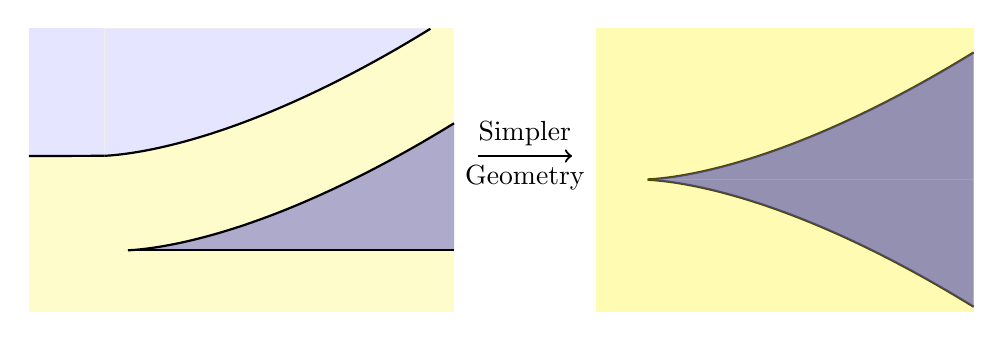
\begin{tikzpicture}[scale=0.6]

\path [fill=blue ,opacity=0.4]
plot [domain=1:70, samples=50, thick ] ( {0.1*\x}, {0.003*pow(\x,1.6)})
|- (0,0);

\path[fill=yellow, opacity=0.2] (-2,-1.3) rectangle (7,4.7);

\path [fill=white]
plot [domain=1:70, samples=50, thick ] ( {0.1*\x-0.5}, {2+0.003*pow(\x,1.6)})
|- (-0.4,4.7);

\path[fill=white, opacity=1] (-2,2) rectangle (-0.4,4.7);

\path [fill=blue, opacity=0.1]
plot [domain=1:70, samples=50, thick ] ( {0.1*\x-0.5}, {2+0.003*pow(\x,1.6)})
|- (-0.4,4.7);

\path[fill=blue, opacity=0.1] (-2,2) rectangle (-0.4,4.7);

\draw [domain=1:70, samples=50, thick] plot( {0.1*\x}, {0.003*pow(\x,1.6)});
\draw [domain=1:70, samples=50, thick] plot( {0.1*\x-0.5}, {2+0.003*pow(\x,1.6)});

\draw [thick] (-2,2) to (-0.4,2.003);
\draw [thick] (0.1,0.003) to (7,0.003);

%%%%%%%%%%%%%%%%%%%%%%%%%%%%%%%%%%%%%%%%%%%%%%%%%%%%%%%%%%%%%%%%%%%%%%%%%%%%%%%%%%%
\draw [thick, ->] (7.5,2) to (9.5,2);
\node at (8.5,2) [above] {Simpler};
\node at (8.5,2) [below] {Geometry};
%%%%%%%%%%%%%%%%%%%%%%%%%%%%%%%%%%%%%%%%%%%%%%%%%%%%%%%%%%%%%%%%%%%%%%%%%%%%%%%%%%

\draw [domain=1:70, samples=50, thick] plot( {11+0.1*\x}, {0.003*pow(\x,1.6)+1.5});
\draw [domain=1:70, samples=50, thick] plot( {11+0.1*\x}, {-0.003*pow(\x,1.6)+1.5});


\path [fill=blue ,opacity=0.6]
plot [domain=1:70, samples=50, thick ] ( {11+0.1*\x}, {0.003*pow(\x,1.6)+1.5})
|- (12,1.5);

\path [fill=blue ,opacity=0.6]
plot [domain=1:70, samples=50, thick ] ( {11+0.1*\x}, {-0.003*pow(\x,1.6)+1.5})
|- (12,1.5);

\path[fill=yellow, opacity=0.3] (10,-1.3) rectangle (18,4.7);


\end{tikzpicture}
\end{document}
